\documentclass[12pt]{rapportINPTCLOUD}
\usepackage{lipsum}
\usepackage{listings}
\title{Rapport INPT CLOUD} %Titre du fichier
\usepackage{lipsum} 
\usepackage{biblatex} %Imports biblatex package
\addbibresource{bibtex.bib} %Import the bibliography file
\usepackage{appendix} % Package pour gérer les annexes
\usepackage{xcolor} % use the color package
\definecolor{chapitrecolor}{RGB}{47, 0, 255} % color of chapitre
\definecolor{sectioncolor}{RGB}{0, 100, 255} % color of section
\definecolor{subsectioncolor}{RGB}{60, 0, 100} % color of subsection
\definecolor{subsubsectioncolor}{RGB}{5, 35, 10} % color of subsubsection
\pagecolor{blue!5!white}
\usepackage{times}
\usepackage{amsmath} 

\begin{document}
	
	%----------- Informations du rapport ---------
	
	\titre{stage à l'hopital} %Title.pdf
	
	\sujet{Rapporte de stage \\ d'initiation} %Subject name
	
	\Encadrants{\textbf{ Leila \textsc{Ennaceur Arjoun}}} %Teacher's name
	
	\eleves{\textbf{Oussama \textsc{Halmous}}} %Students
	
	%----------- Initialisation -------------------
	
	\fairemarges %Afficher les marges
	\fairepagedegarde %Créer la page de garde
	\setlength{\baselineskip}{0.35in}
	\newpage
	\begin{center}
		\Huge{ REMERCIEMENTS }
	\end{center}
	\begin{center}
		Madame Leila ENNACEUR  ARJOUN,\\
	
	Par la présente, je tiens à vous exprimer mes sincères remerciements pour votre encadrement et votre soutien précieux durant mon stage d'initiation au sein du département d'informatique.
	
	------
	
	Votre expertise et votre dévouement m'ont permis d'acquérir des connaissances et des compétences inestimables dans le domaine d'informatique. 
	
	-------------
	
	Je suis convaincu(e) que les expériences et les compétences que j'ai acquises lors de ce stage me seront d'une grande utilité pour la suite de mon parcours professionnel.
	
	----------------------
	
	Je vous remercie encore une fois pour votre générosité et votre contribution à mon développement personnel et professionnel.
	
	\end{center}
	
	
	\tabledematieres %Créer la table de matières
	\listoffigures
	%\listoftables
	\newpage
\begin{center}
	\texttt{	"Si on me le dit, j’oublie. Si on me le montre, je me souviens. Si on m’implique, j’apprends."}
\end{center}
	
	Cette citation d’un écrivain français met en évidence l’importance de l’implication pour toute personne souhaitant aiguiser ses connaissances.
	
	En effet, le stage est une période importante dans la vie d’un étudiant, car il lui permet de confronter directement ses connaissances théoriques aux savoir-faire exigés par le monde professionnel.
	
	Consciente de cette importance, l’Institut Supérieur des Etudes Technologiques de Médenine a introduit, dans le cadre de ses programmes, un stage d’une durée d’un mois destiné aux étudiants de première année leur offrant l’opportunité de mettre à l’épreuve leurs connaissances acquises à l’ISET\footnote{ISET : Institut Supérieur des Etudes Technologiques} Médenine en les confrontant aux problèmes concrets auxquels est confrontée l’entreprise pour aboutir à la rédaction d’un mémoire de fin d’études.
	
	En ce qui me concerne, j’ai eu l’opportunité de réaliser mon stage au sein de l’hôpital Habib Bourguiba de Médenine, l’établissement sanitaire leader dans la région de Médenine.
	Mon sujet s’articule autour de l’évaluation du système d’information hospitalier de l’hôpital Habib Bourguiba de Médenine, ce sujet étant en lien avec les besoins actuels que vit l’établissement.
	
	Le sujet répond parfaitement à mes attentes et à ma grande volonté d’aborder un sujet qui se focalise sur le système d’information sanitaire (SIS) . 
	
	J’ai pu atteindre tous mes objectifs de stage. J’ai pu mettre en pratique mes connaissances acquises en matière de SIH, acquérir de nouvelles compétences en matière de SIH, et apprendre que j’ai un esprit d’analyse et de synthèse.
	\newpage
	\setcounter{page}{1}
	\chapter*{Introduction générale}
		\begin{center}

		Le Système d'Information Sanitaire ,
	\end{center}
	\begin{center}
		\texttt{Vers une Numérisation Complète du Secteur de la Santé}
	\end{center} 
	
	En Tunisie, le Centre national d'informatique sanitaire (CIMS) s'engage dans un projet ambitieux : la mise en place d'un Système d'Information Sanitaire (SIS) national intégré. Ce système vise à révolutionner la gestion du secteur de la santé en numérisant l'ensemble des transactions, des données patients aux aspects financiers et administratifs.\\
	
	Plus qu'une simple numérisation, ce projet représente une transformation profonde du système de santé tunisien. Il s'agit de créer un environnement numérique intégré et interopérable, capable de collecter, stocker, traiter et analyser l'ensemble des données relatives à la santé de la population.\\
	
	\begin{figure}[H]
		\centering
		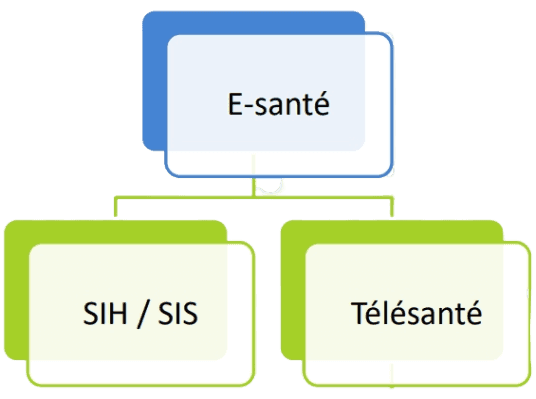
\includegraphics[width=1\linewidth]{img/m-sih-sis.png}
		\caption{le système d'information sanitaires "e-santé"}
		\label{fig:e-santé}
	\end{figure}
	
	\chapter{\textcolor{chapitrecolor}{Système d'Information Hospitalier}}
	
	Le SIS\footnote{SIS : Système d'Information Sanitaire} est un ensemble d'outils numériques qui permettent la gestion, le stockage et l'échange d'informations relatives à la santé des individus. Il relie les différents acteurs du système de santé, tels que les médecins, les hôpitaux, les pharmacies et les organismes d'assurance maladie.
	On peut dire qu’un SIH\footnote{SIH : Système d'Information Hospitalier} est un des élements du SIS plus vaste .
	
	Un SIH est un ensemble de ressources informatiques et humaines permettant de collecter, de traiter et de diffuser des informations nécessaires à la gestion d'un établissement hospitalier. Il est composé de différents composants, qui interagissent entre eux pour fournir un système complet et intégré.
	\section{Definition}
	
	Le SIH est un ensemble d'outils numériques qui permettent la gestion, le stockage et l'échange d'informations relatives à la santé des individus. Il s'agit d'un élément essentiel du système de santé, reliant les différents acteurs tels que les médecins, les hôpitaux, les pharmacies et les organismes d'assurance maladie.	
	\section{Composants du SIH}
	
	Le SIH est composé de plusieurs modules qui interagissent entre eux pour fournir un système complet et intégré. Les principaux modules sont les suivants:
	
	\begin{itemize}
		\item[>] 	Système d'Information de Gestion Hospitalière (SIGH): Il gère les aspects administratifs de l'hôpital, tels que la facturation, la gestion des stocks et des ressources humaines.
		\item[>] 	Système d'Information Médico-Administratif (SIMA): Il stocke et gère les informations administratives des patients, telles que leurs coordonnées, leur historique médical et leurs allergies.
		\item[>] 	Système d'Information Médical (SIM): Il gère les informations cliniques des patients, tels que les résultats de laboratoire, les images médicales et les prescriptions.
		\item[>] 	Système d'Information Médico-Economique (SIME): Il fournit des informations sur les activités et les coûts des structures hospitalières.
		\item[>] 	Système d'Information de Pilotage et d'Aide à la Décision (SIPAD): Il permet de suivre les performances de l'hôpital et d'identifier les axes d'amélioration.
		\item[>] 	Système d'Information des SAMU (SI-SAMU): Il optimise la gestion des interventions et du travail au sein des services d'aide médicale urgente.
	\end{itemize}
	
	
	\section{Avantages du SIH}
	
	Le SIH présente de nombreux avantages pour les patients, les professionnels de santé et les gestionnaires d'hôpitaux.
	
	\begin{itemize}
		
		\item[*]  Pour les patients:
		
		\begin{itemize}
			\item[.] 		Amélioration de la qualité des soins
			\item[.] 		Réduction des erreurs médicales
			\item[.] 		Accès plus facile aux informations médicales
			\item[.] 		Simplification des démarches administratives
		\end{itemize}
		
		\item[*] Pour les professionnels de santé:
		
		\begin{itemize}
			\item[.] 		Amélioration de la communication et de la collaboration
			\item[.] 		Accès plus facile aux informations patient
			\item[.] 		Gain de temps et d'efficacité
		\end{itemize}
		
		\item[*] Pour les gestionnaires d'hôpitaux:
		
		\begin{itemize}
			\item[.] 		Réduction des coûts
			\item[.] 		Meilleure prise de décision
			\item[.] 		Amélioration de la performance
		\end{itemize}
		
	\end{itemize}
	
	\section{Conclusion}
	
	Le SIH est un outil essentiel pour l'amélioration de la qualité des soins et de l'efficacité du système de santé. Enjeu majeur pour l'avenir de la santé, il continuera à se développer et à se perfectionner pour répondre aux besoins croissants des patients et des professionnels de santé.
	\chapter{\textcolor{chapitrecolor}{Les applications du SIH}}
	Le CIMS joue un rôle crucial dans la modernisation du système de santé tunisien en concevant et en développant des applications informatiques innovantes pour le Ministère de la Santé. Ces applications, regroupées sous le Système d'Information Hospitalier (SIH), visent à améliorer l'efficacité, la qualité et la coordination des soins au sein des hôpitaux et des services de santé.
	
	Le SIH offre une large gamme d'applications couvrant divers aspects de la gestion hospitalière, notamment :
	\section{\textcolor{sectioncolor}{les applications de gestion des malades :}}
	\subsection{Soins :} Inscription aux consultations externes et aux urgences, planification des rendez-vous, suivi des dossiers patients.
	\begin{figure}[H]
		\centering
		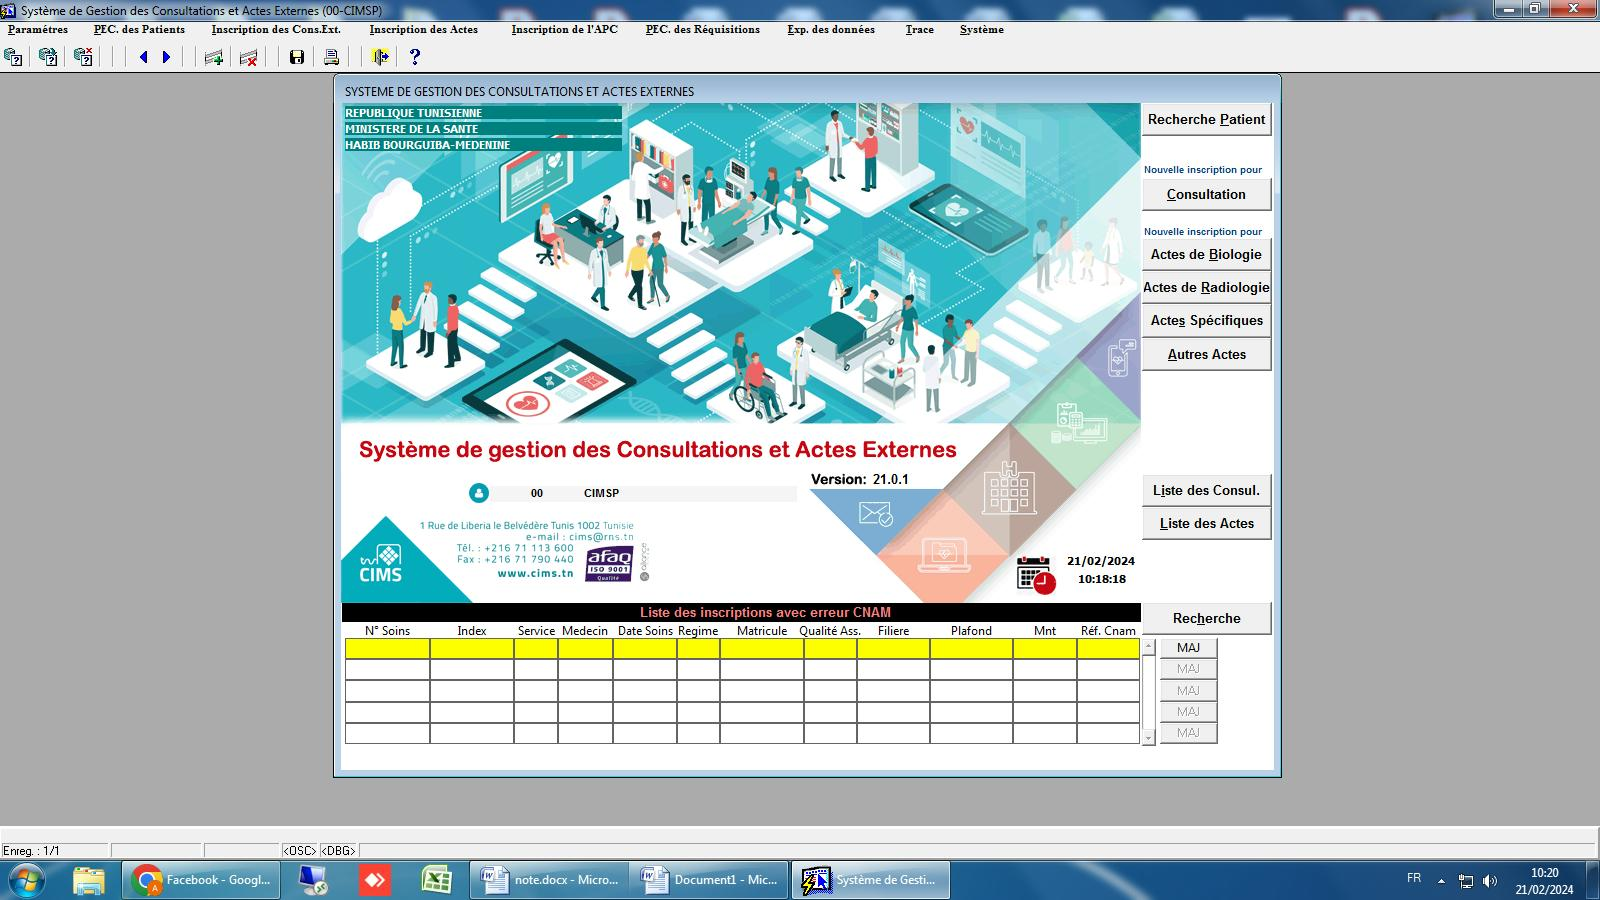
\includegraphics[width=1\linewidth]{img/a.jpg}
		\caption{l'application Soins}
		\label{fig:Soins}
	\end{figure}	
\newpage
\subsection{admiss :} Gestion des hospitalisations, planification des lits, suivi des patients hospitalisés.
\begin{figure}[H]
\centering
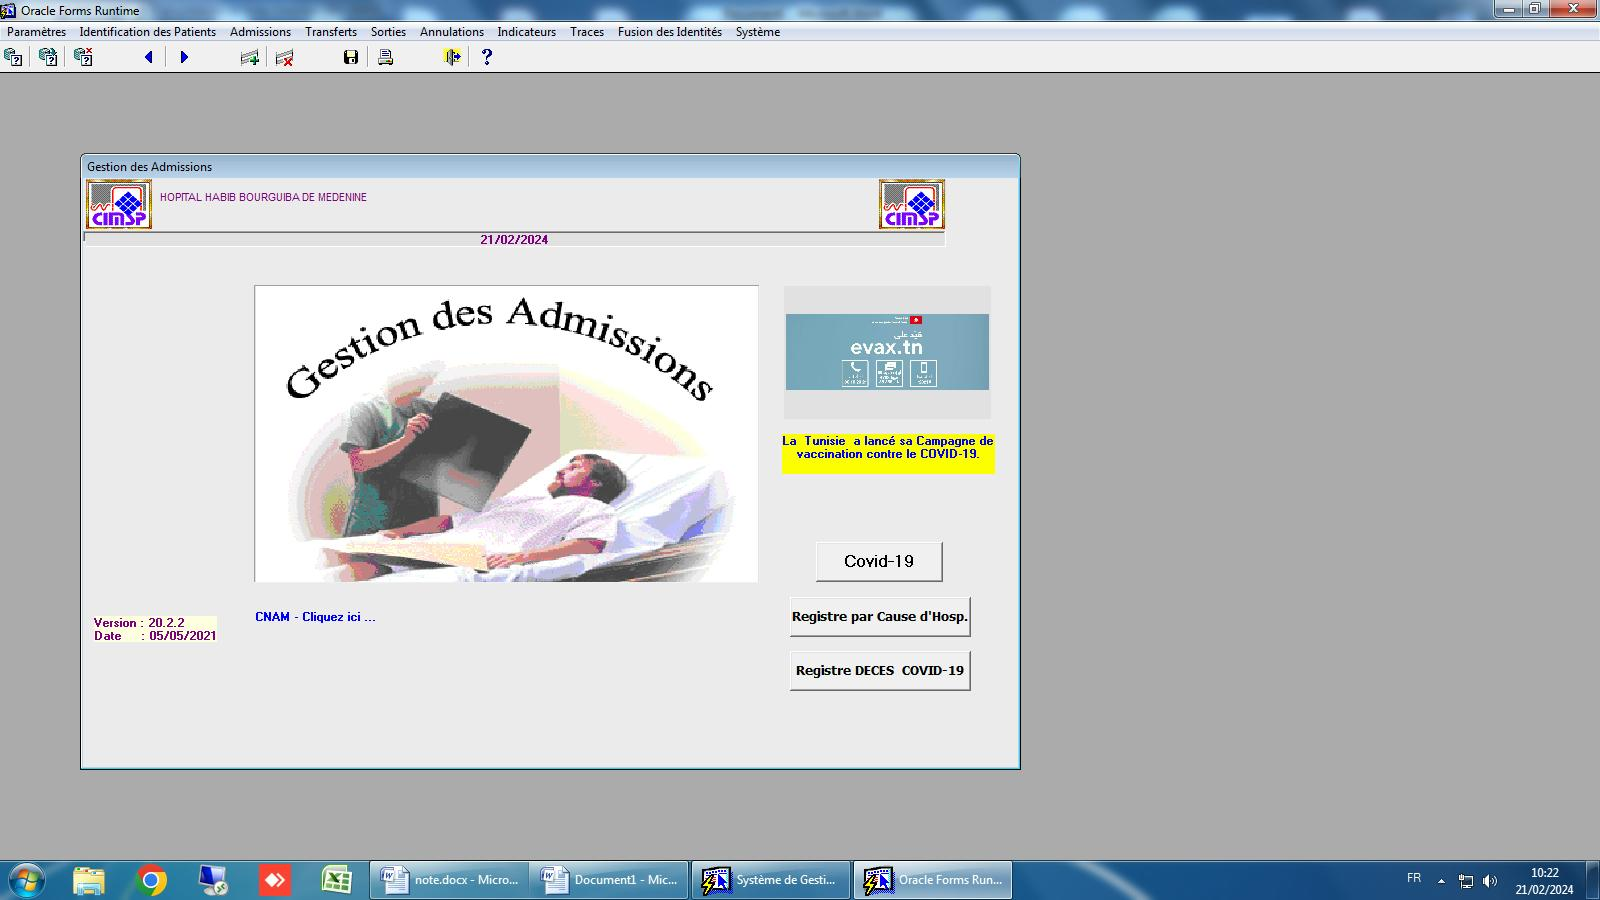
\includegraphics[width=1\linewidth]{img/b.jpg}
\caption{l'application admiss}
\label{fig:admiss}
\end{figure}

\subsection{facture :}  Facturation des frais médicaux, génération des reçus, gestion des paiements.
\begin{figure}[H]
\centering
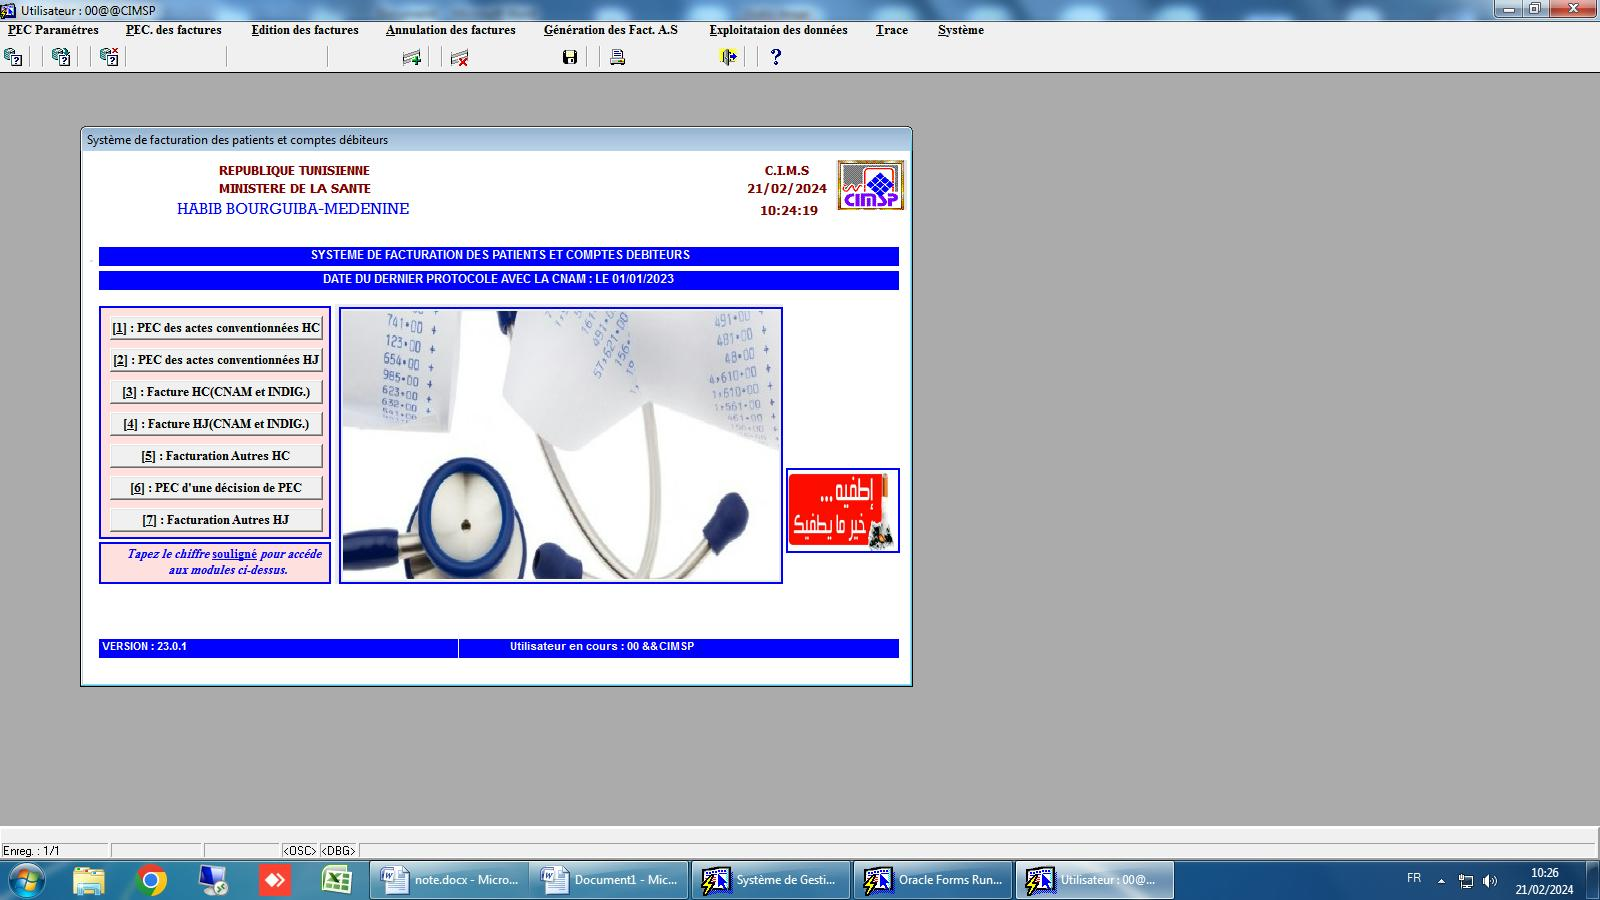
\includegraphics[width=1\linewidth]{img/c.jpg}
\caption{l'application facture}
\label{fig:facture}
\end{figure}

\subsection{finances :} Gestion des recettes et des dépenses, suivi budgétaire, comptabilité.
\begin{figure}[H]
\centering
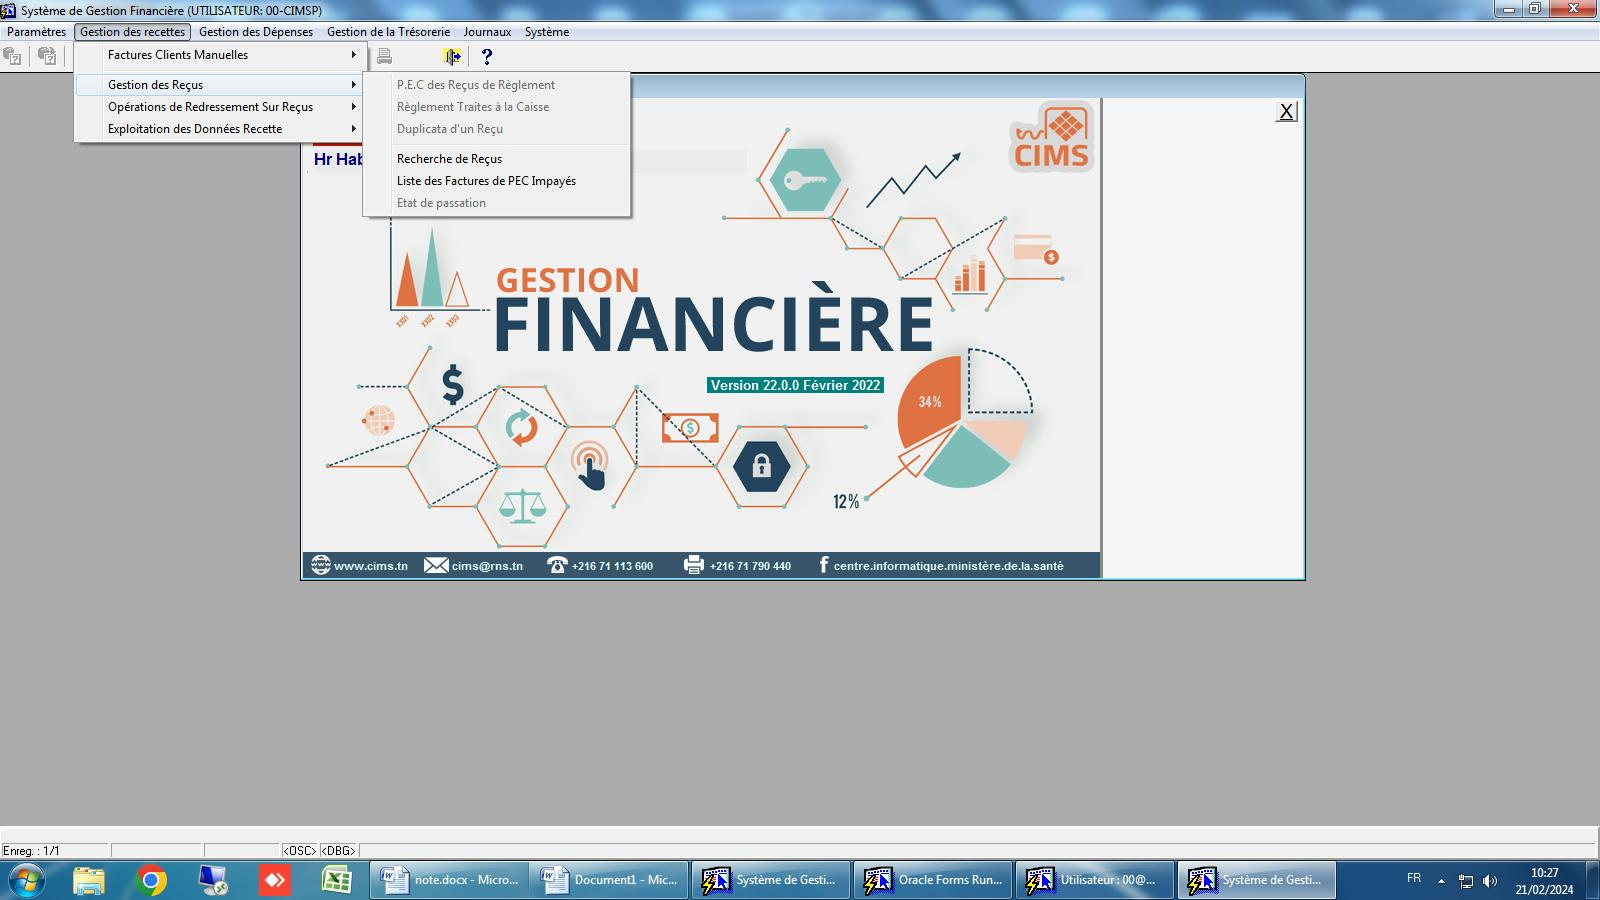
\includegraphics[width=1\linewidth]{img/d.jpg}
\caption{l'application finances}
\label{fig:finances}
\end{figure}
\newpage
	\section{\textcolor{sectioncolor}{les applications d’approvisionnement :}}
\subsection{achat :}   Gestion des commandes externes d'articles, de travaux et d'équipements
\begin{figure}[H]
	\centering
	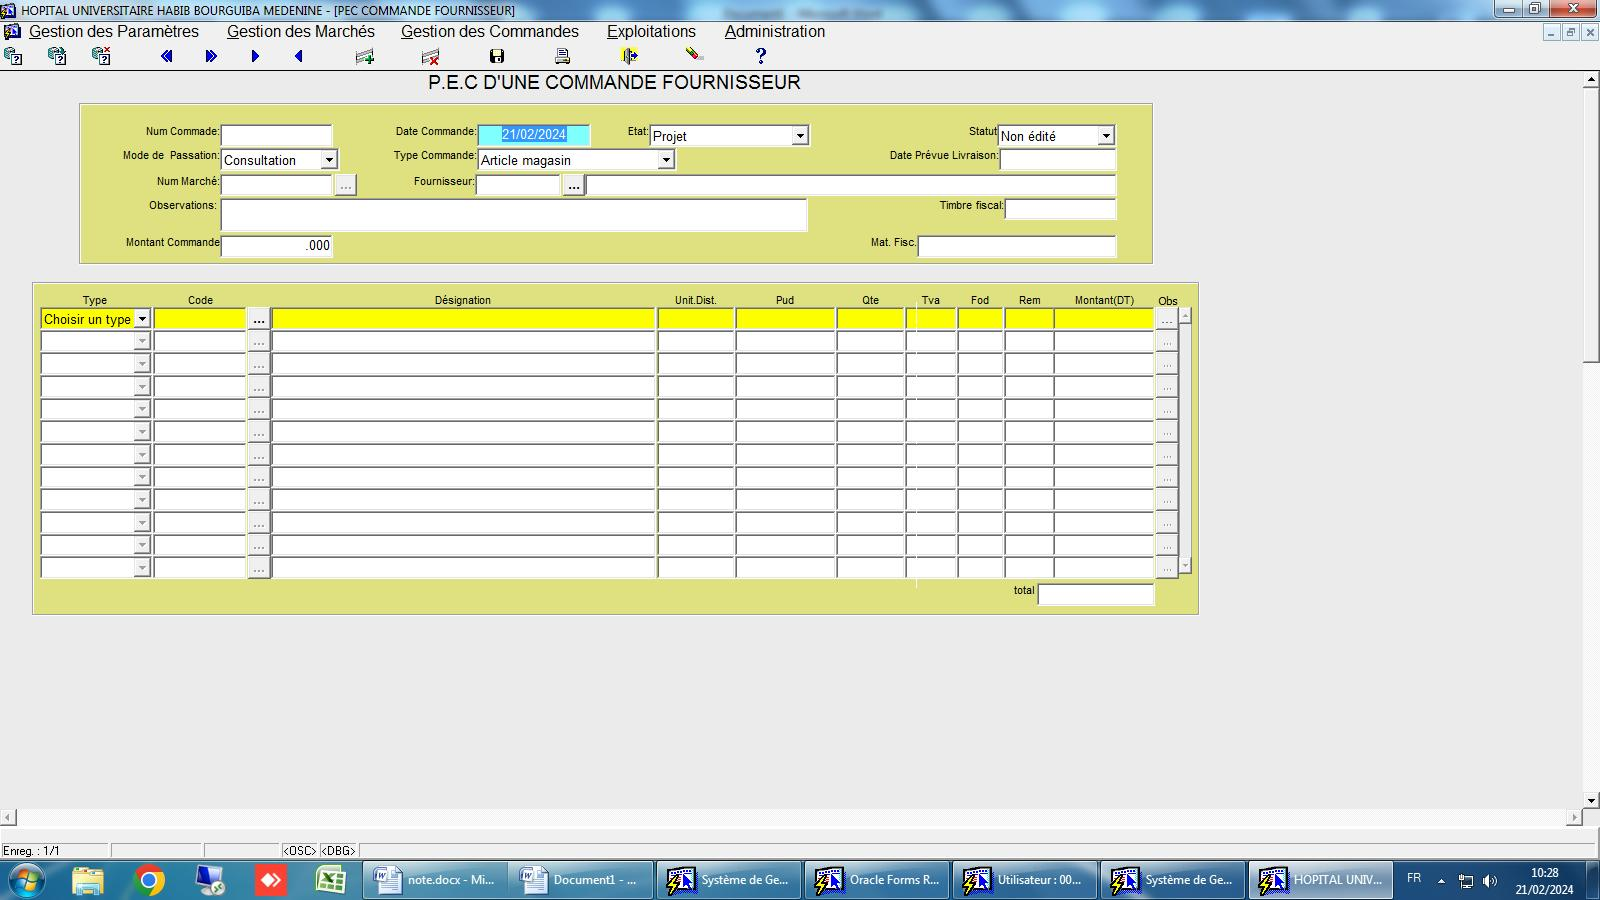
\includegraphics[width=1\linewidth]{img/e.jpg}
	\caption{l'application achat}
	\label{fig:achat}
\end{figure}
\newpage
\subsection{STKMAG :} Gestion du stock magasin en équipements et en articles, inventaires, suivi des stocks.
\begin{figure}[H]
	\centering
	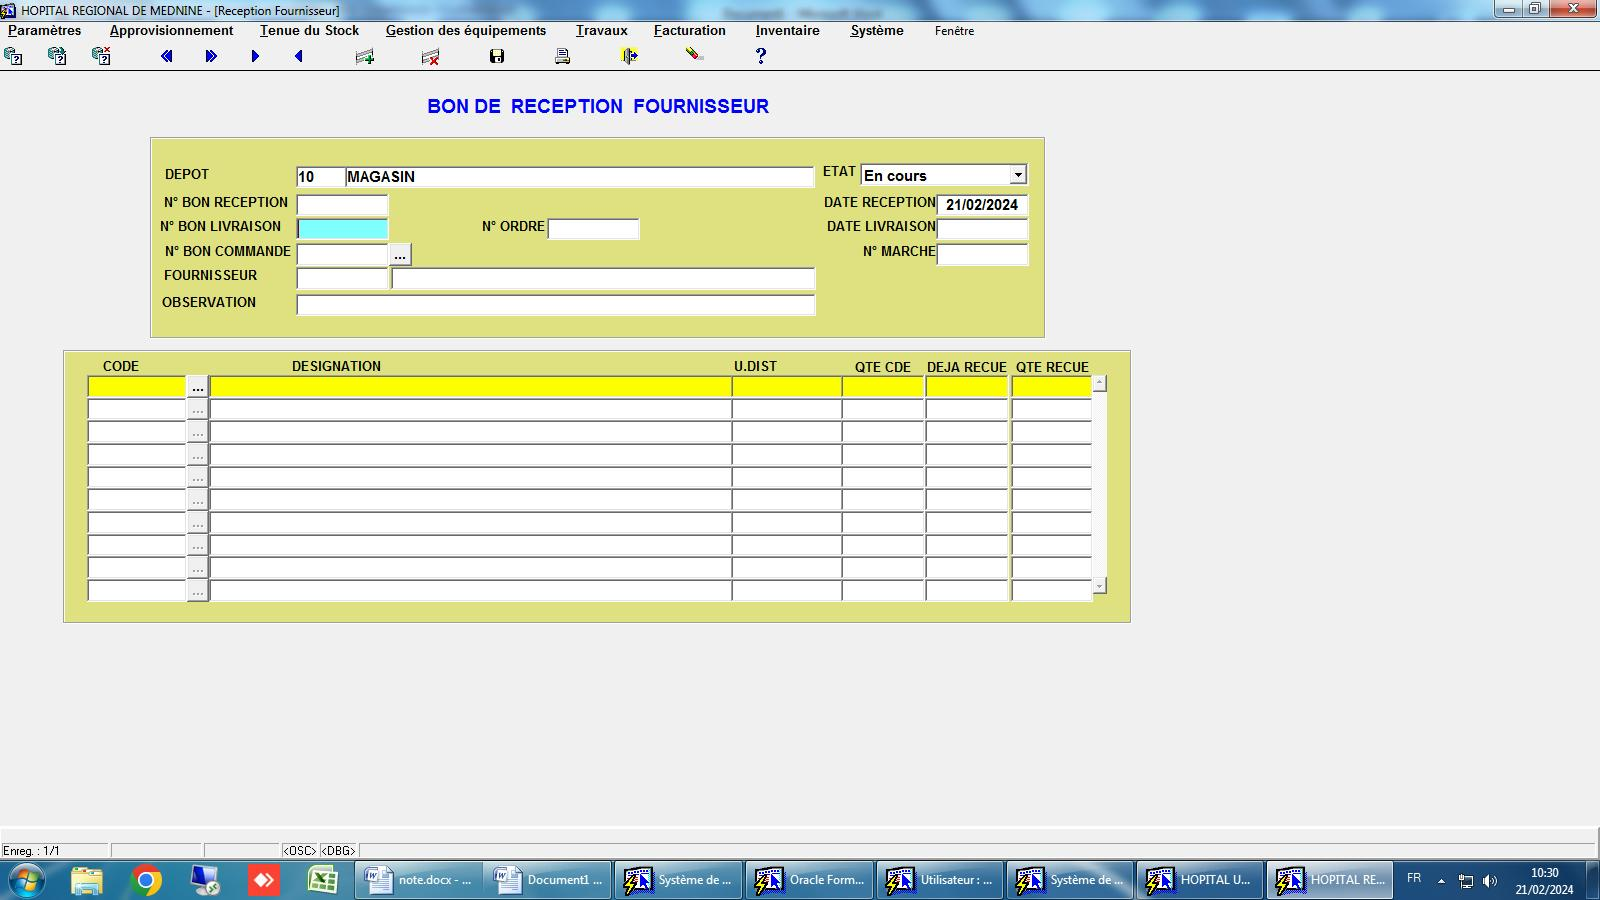
\includegraphics[width=1\linewidth]{img/f.jpg}
	\caption{l'application STKMAG}
	\label{fig:STKMAG}
\end{figure}

\subsection{Bon de Prélevement (BP) :} Gestion des commandes internes dans l'hôpital, suivi des transferts de stocks.
\begin{figure}[H]
	\centering
	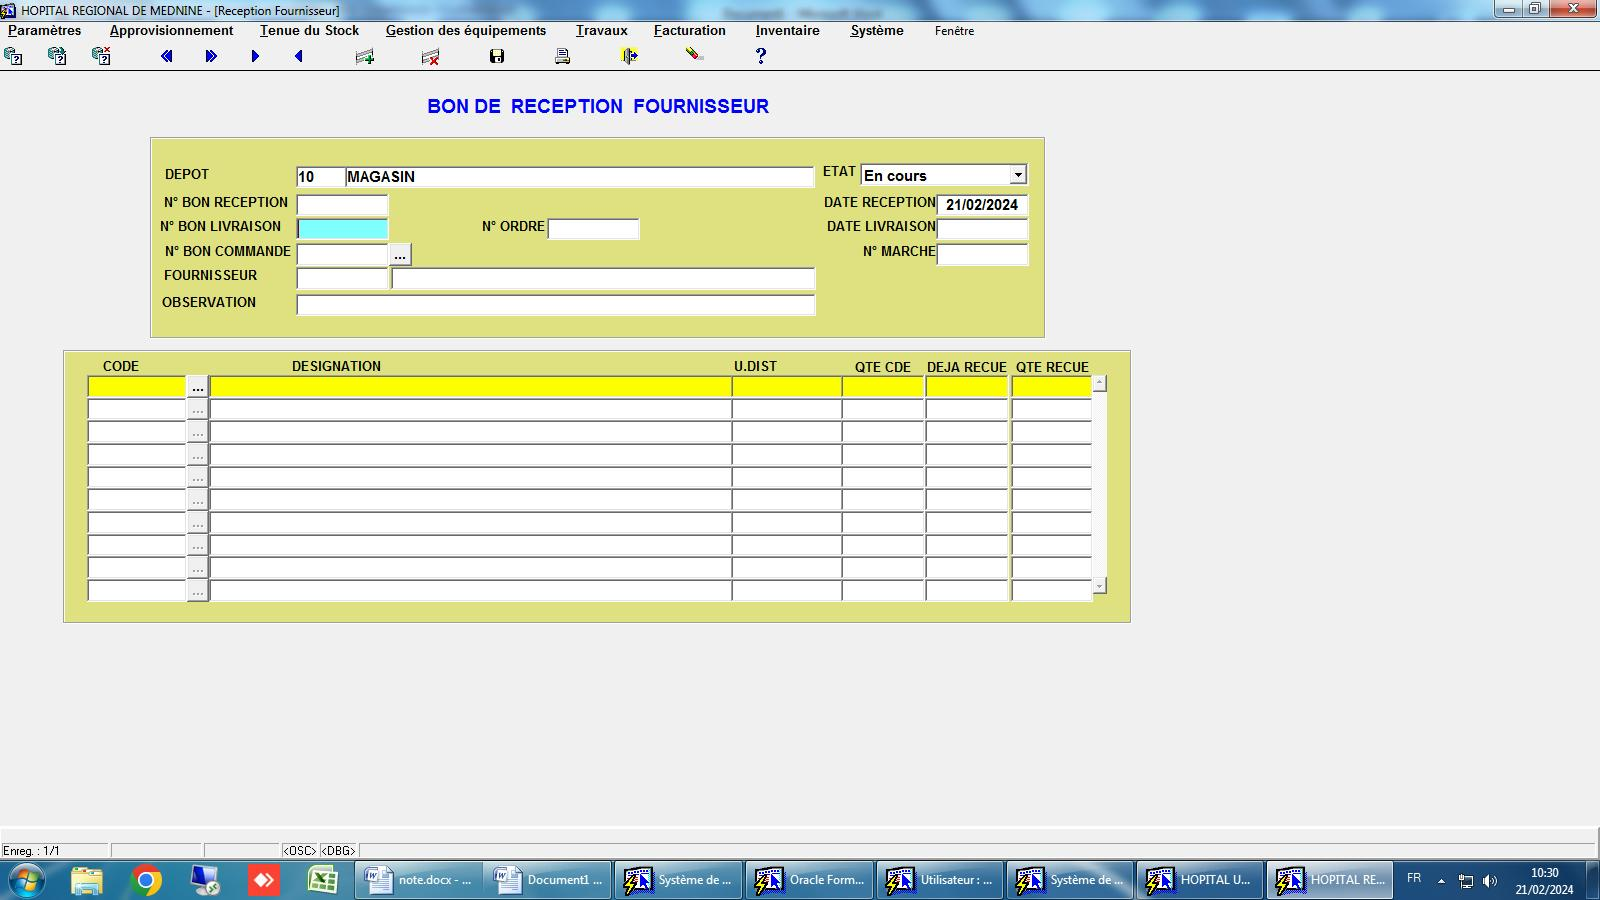
\includegraphics[width=1\linewidth]{img/g.jpg}
	\caption{l'application Bon de Prélevement}
	\label{fig:Bon de Prélevement}
\end{figure}
	\section{\textcolor{sectioncolor}{les applications des services annexes :}}

\subsection{Santelab :}   gestion des demandes et résultats des analyses dans le laboratopire de biologie 
\begin{figure}[H]
	\centering
	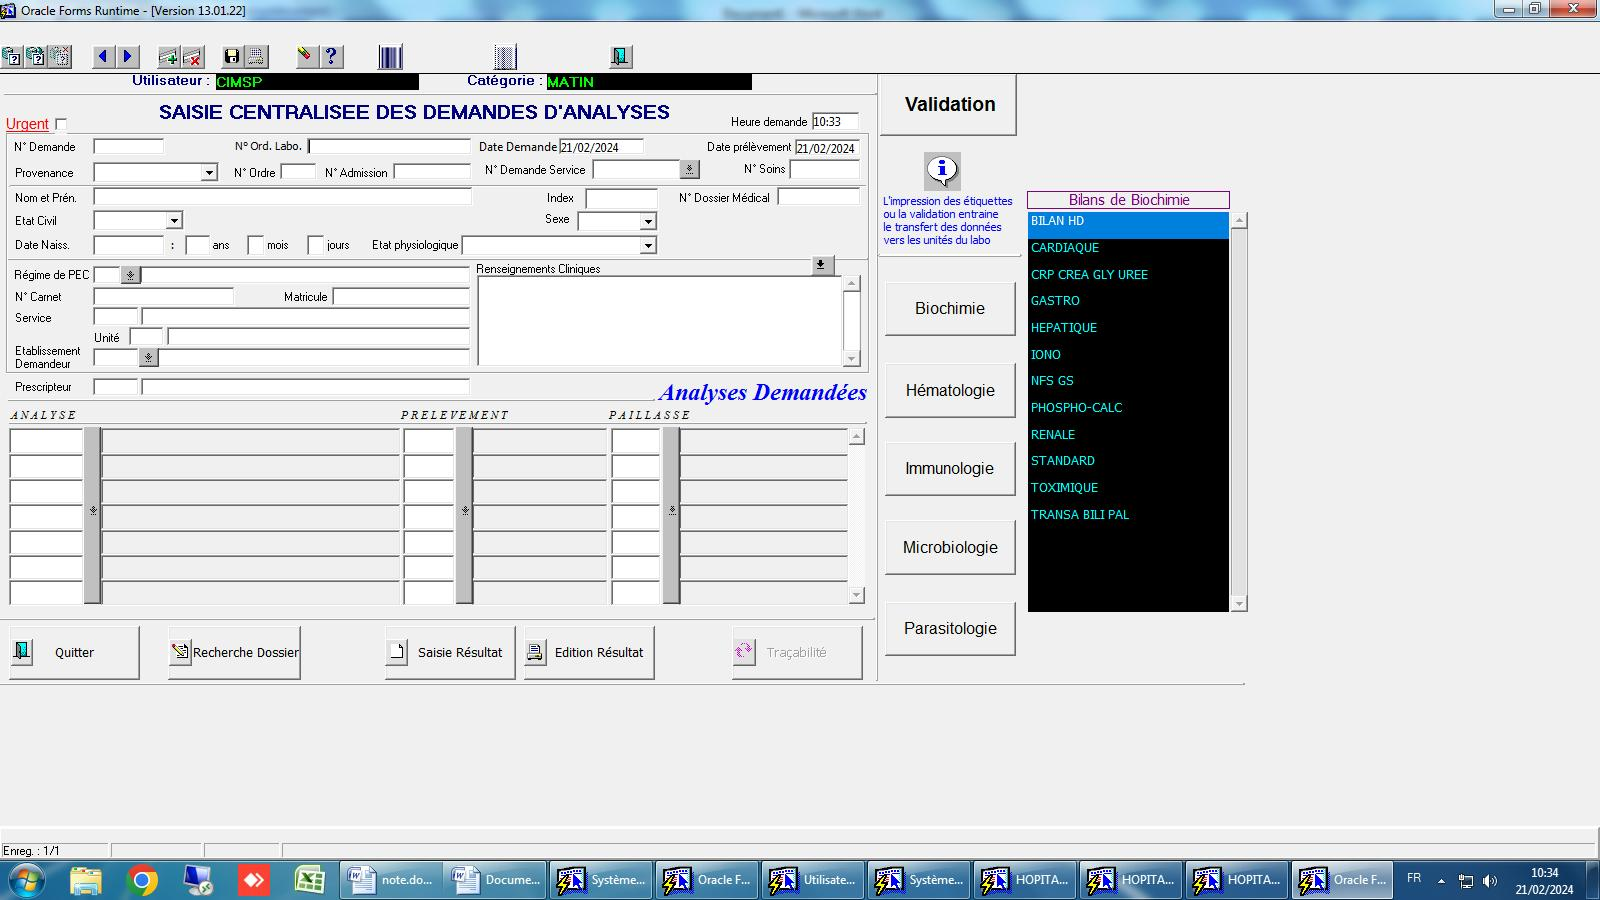
\includegraphics[width=1\linewidth]{img/h.jpg}
	\caption{l'application Santelab}
	\label{fig:Santelab}
\end{figure}
\newpage
\subsection{Anapth :} gestion des demandes et résultats des analyses dans le laboratoire d’analyses pathlogiques 
\begin{figure}[H]
	\centering
	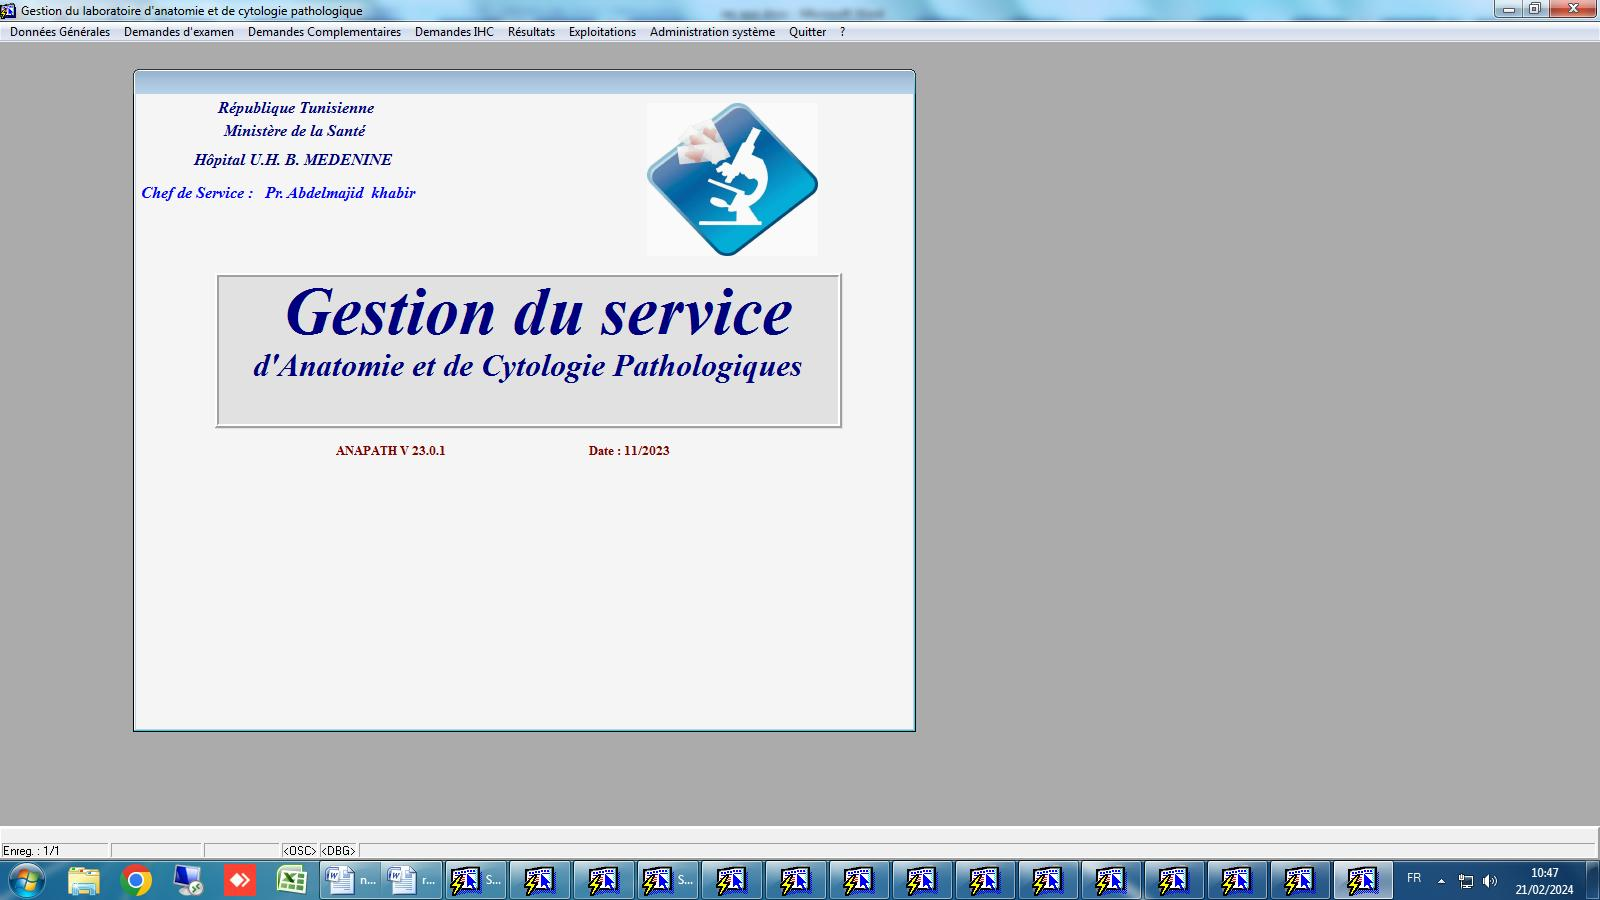
\includegraphics[width=1\linewidth]{img/i.jpg}
	\caption{l'application Anapth}
	\label{fig:Anapth}
\end{figure}

\subsection{Radio :}   gestion des demandes des actes de radios, des scanneur, des IRM et des echographies
\begin{figure}[H]
	\centering
	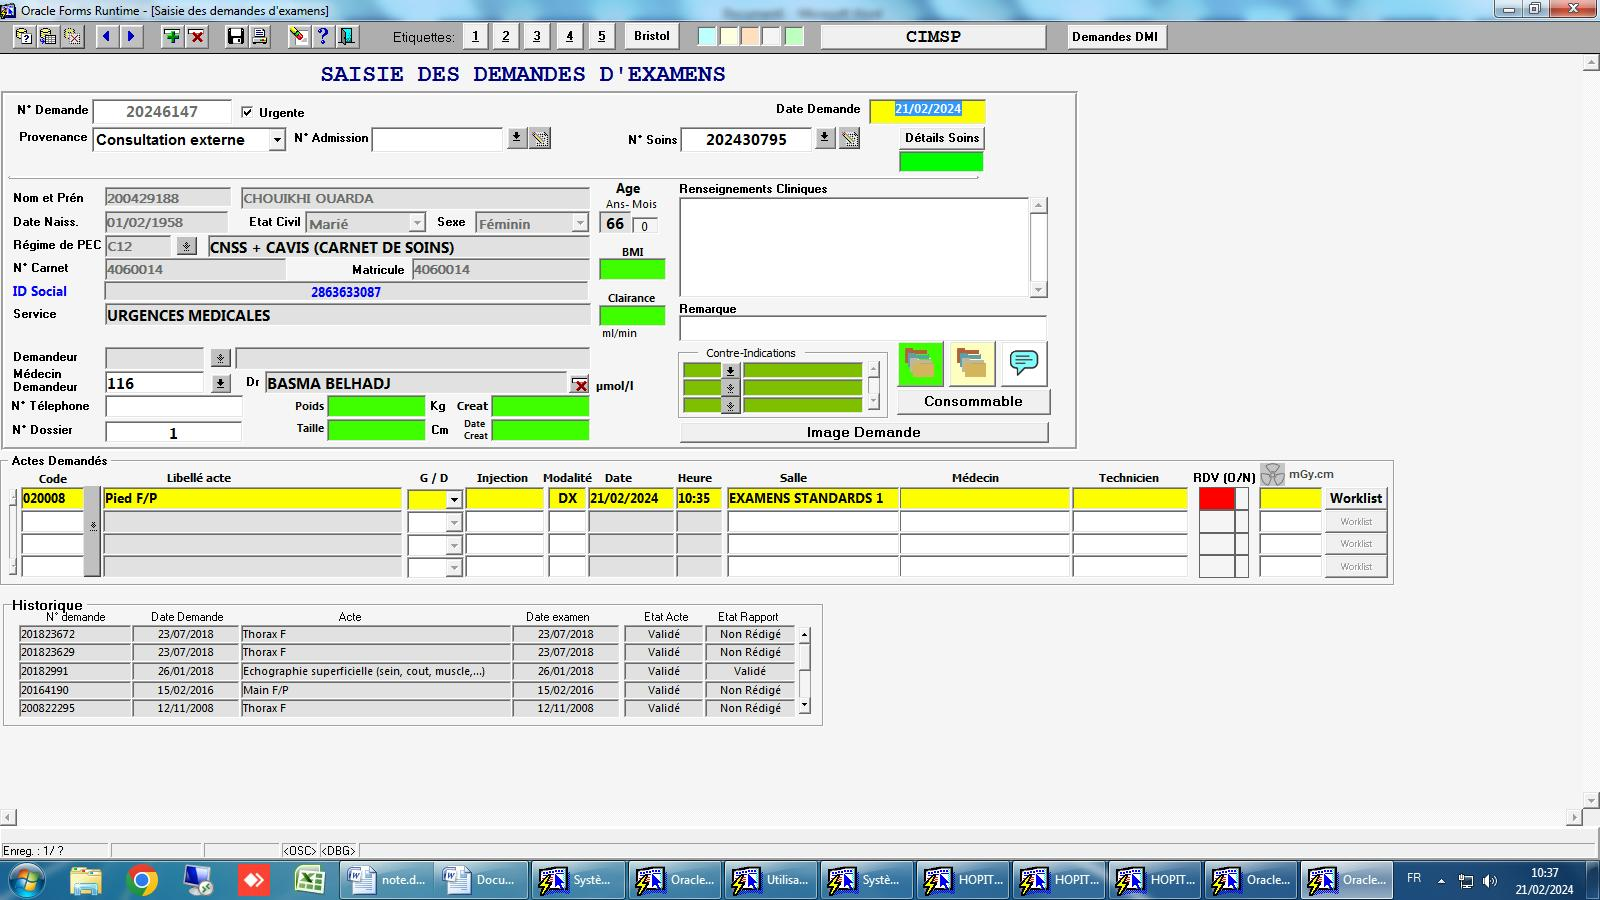
\includegraphics[width=1\linewidth]{img/j.jpg}
	\caption{l'application Radio}
	\label{fig:Radio}
\end{figure}

\subsection{biomed :}  Gestion du parc biomédical (tous les équipements biomédicaux et automates), maintenance, suivi des interventions.
\begin{figure}[H]
	\centering
	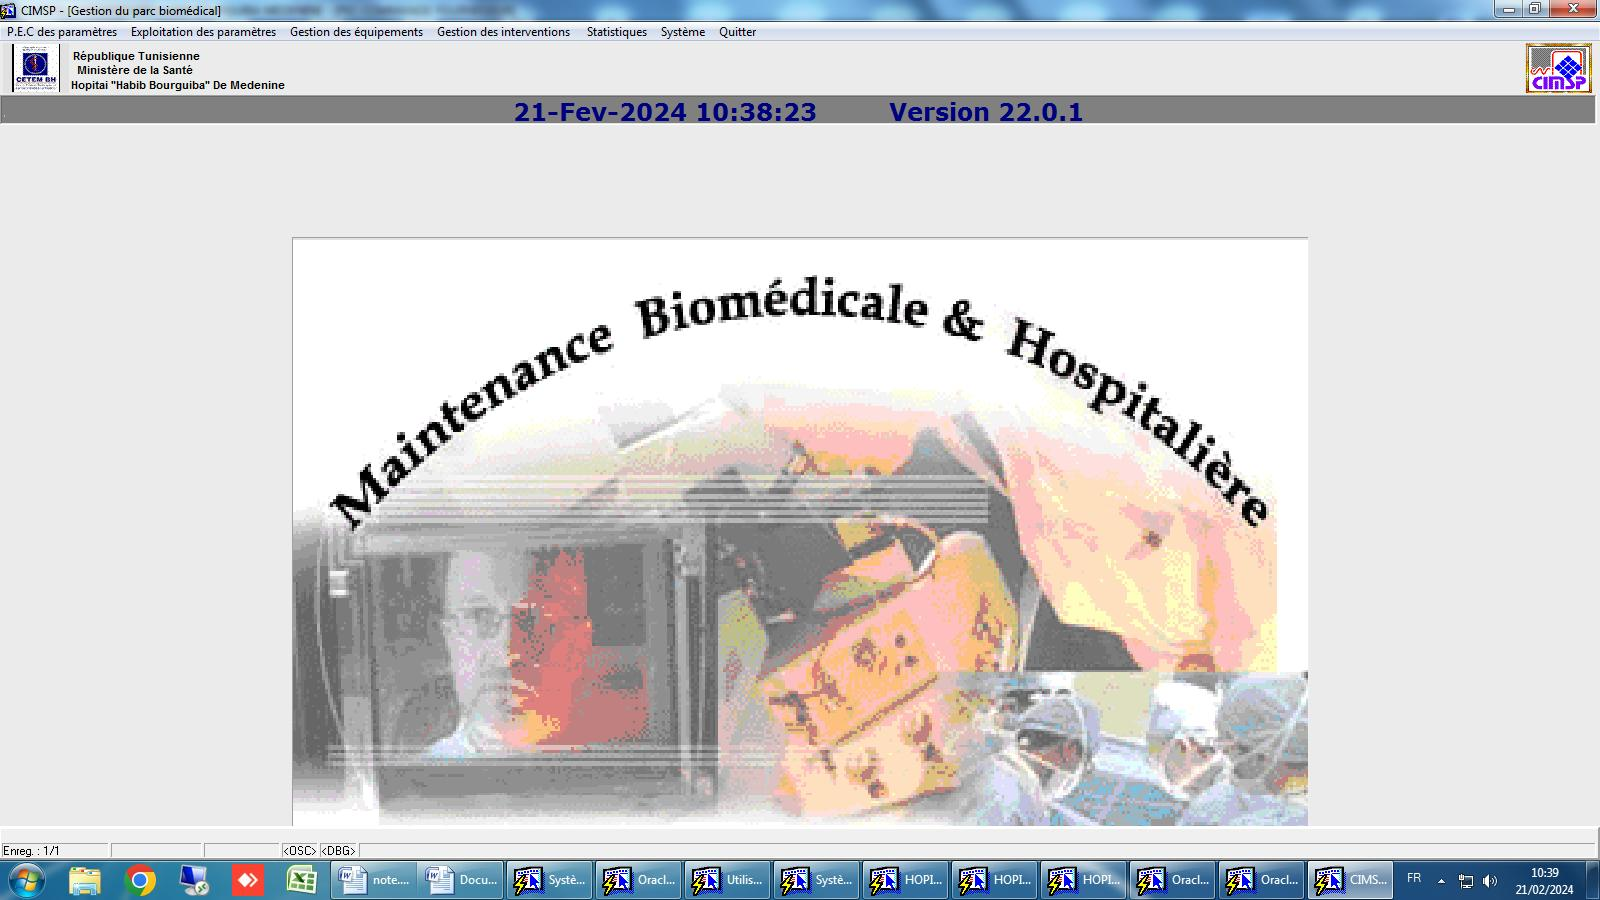
\includegraphics[width=1\linewidth]{img/k.jpg}
	\caption{l'application biomed}
	\label{fig:biomed}
\end{figure}
\newpage
	\section{\textcolor{sectioncolor}{l'application du Dossier Médical Informatisé (DMI) :}}
	
	Collecte des données relatives au patient lors de tout accès dans l'hôpital, historique des services fréquentés.
\begin{figure}[H]
	\centering
	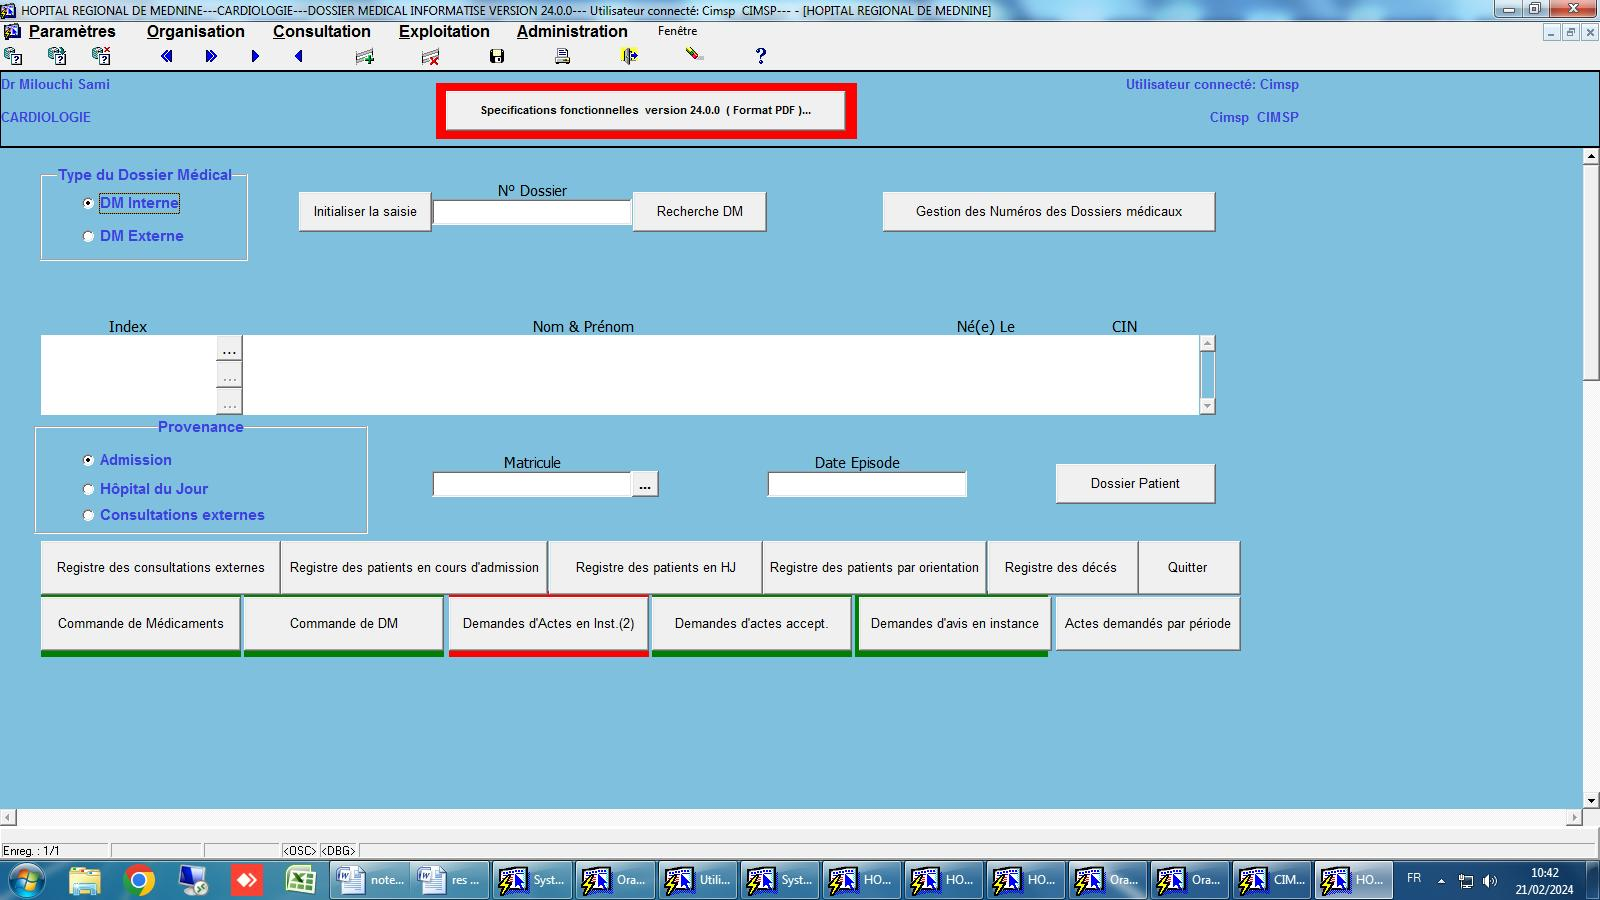
\includegraphics[width=1\linewidth]{img/l.jpg}
	\caption{l'application Dossier Médical Informatisé}
	\label{fig:Dossier Médical Informatisé}
\end{figure}\newpage
	\section{\textcolor{sectioncolor}{la gestions du stock des médicaments :}}

\subsection{STKMED :} Gestion du stock des médicaments, inventaires, suivi des péremptions.
\begin{figure}[H]
	\centering
	
\includegraphics[width=1\linewidth]{img/m.jpg}
	\caption{l'application STKMED}
	\label{fig:STKMED}
\end{figure}
 .\\ \\ \\
\subsection{ACCESS :} Gestion du stock des accessoires médicaux, inventaires, suivi des stocks.
\begin{figure}[H]
	\centering
	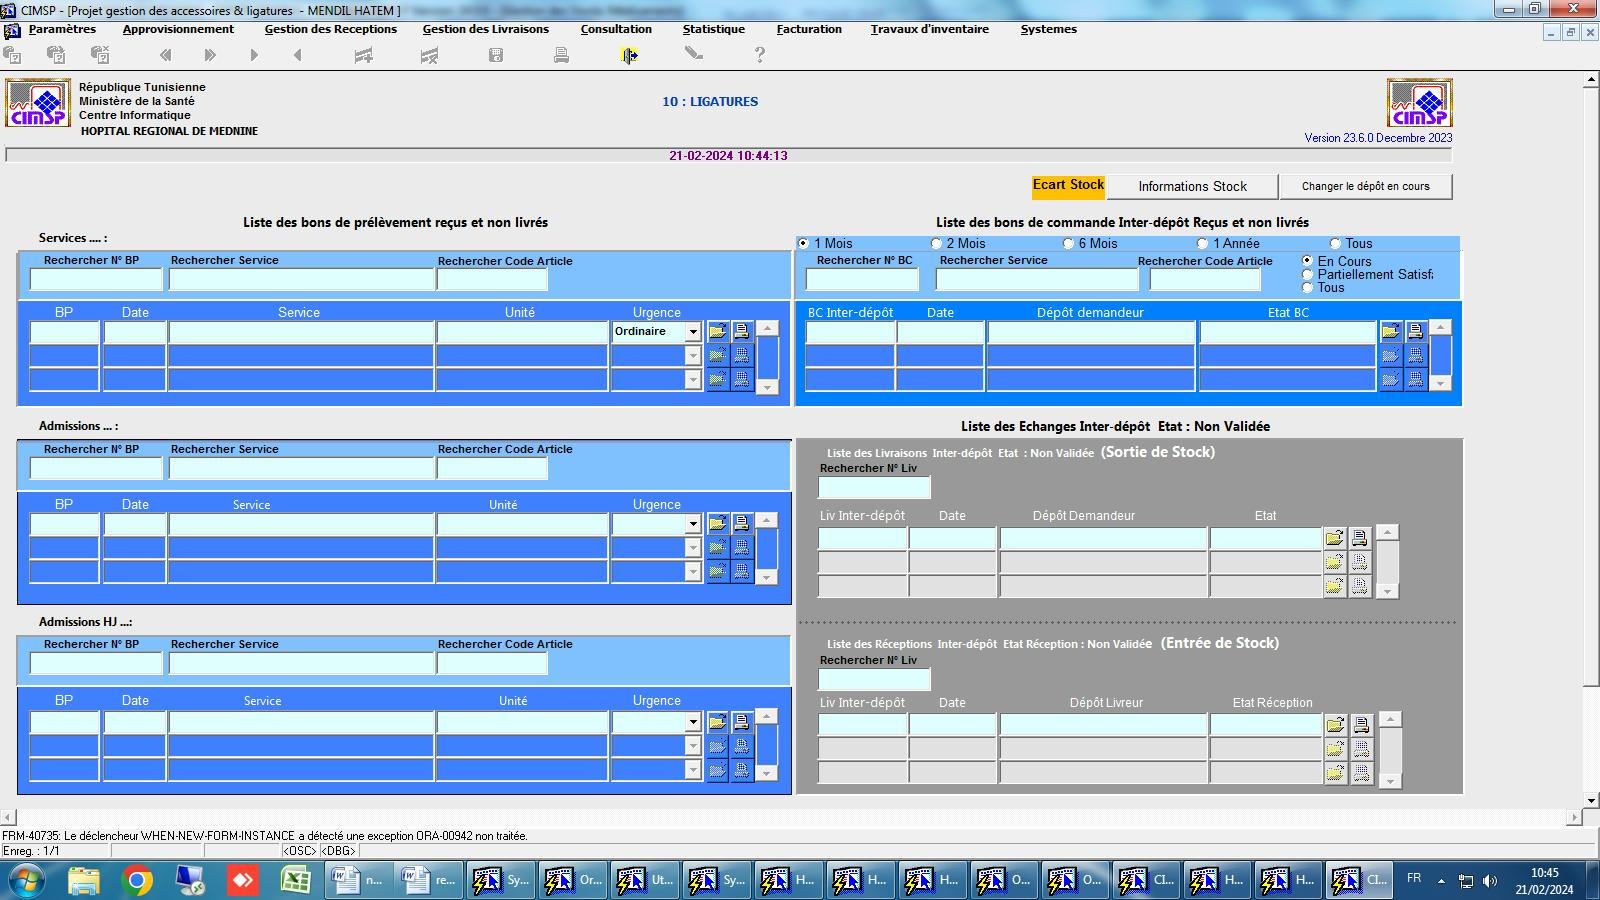
\includegraphics[width=1\linewidth]{img/n.jpg}
	\caption{l'application ACCESS}
	\label{fig:ACCESS}
\end{figure}

 

	\section{\textcolor{sectioncolor}{l'application dialyses :}}

Gestion des séances de dialyse pour les patients affiliés à la CNAM, planification des séances.

\begin{figure}[H]
	\centering
	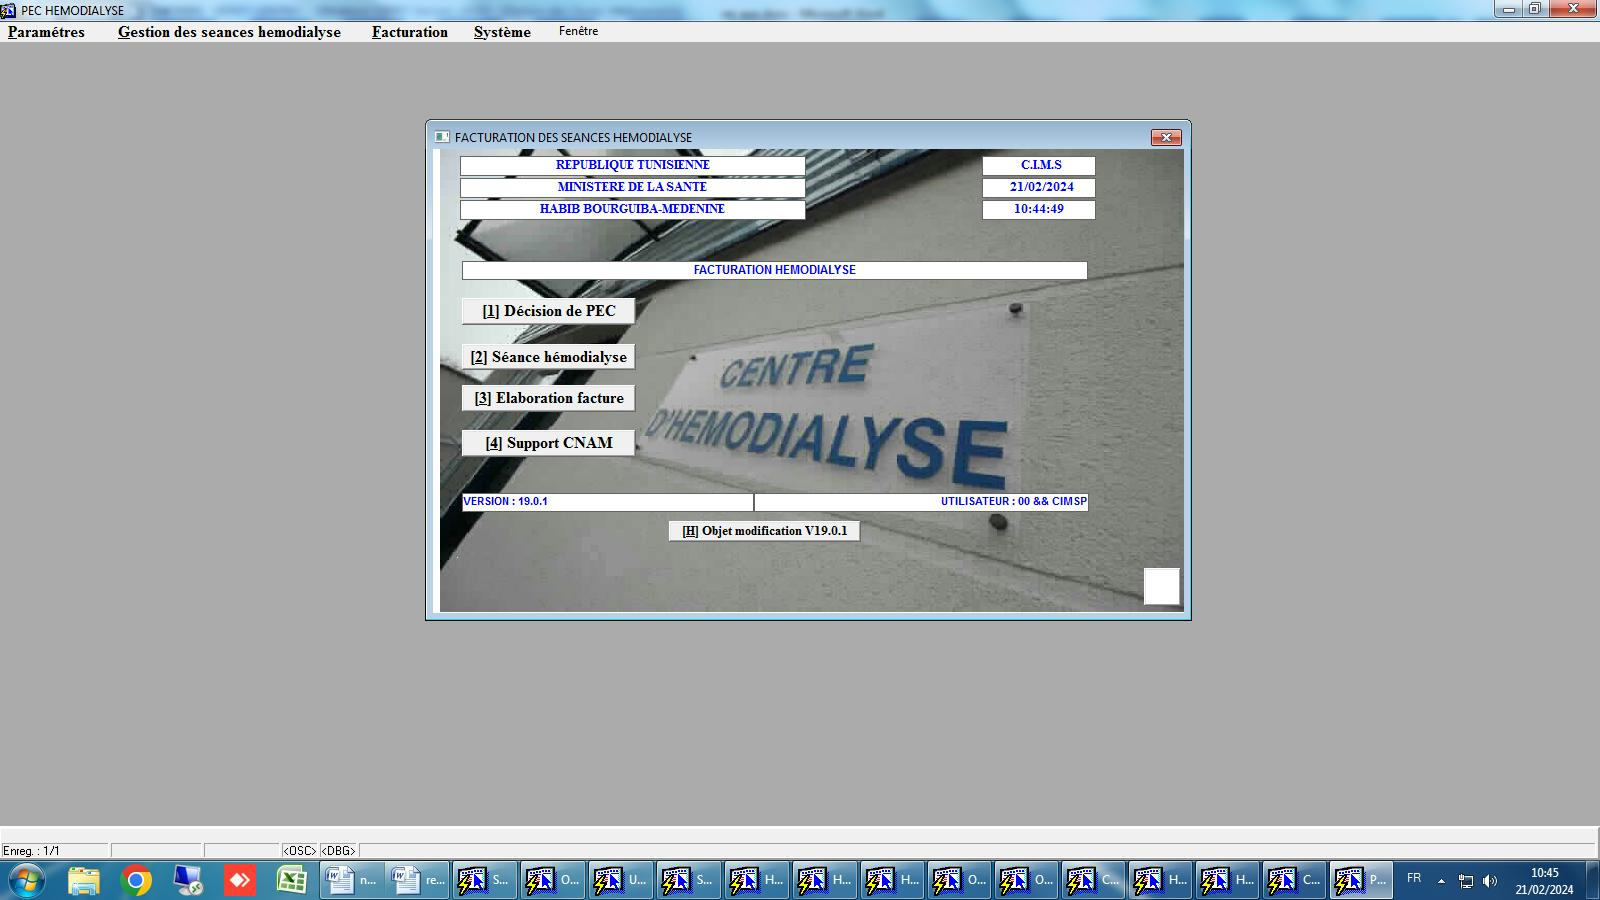
\includegraphics[width=1\linewidth]{img/o.jpg}
	\caption{l'application dialyses}
	\label{fig:dialyses}
\end{figure}
.\\ \\ \\ 
Le développement et la mise en place du Système d'Information Hospitalier (SIH) par le Centre Informatique du Ministère de la Santé (CIMS) constituent une avancée majeure pour le système de santé tunisien. Le SIH offre une large gamme d'applications qui permettent d'améliorer l'efficacité, la qualité et la coordination des soins au sein des hôpitaux et des services de santé.

\begin{center}
	\Huge{Conclusion générale}
\end{center}
\large {
Le système d'information hospitalier (SIH) est un outil essentiel pour la gestion efficace d'un hôpital. Il permet d'améliorer la coordination des soins aux patients, de réduire les erreurs médicales, d'améliorer la communication entre les professionnels de santé et de gagner du temps et de l'argent.\\

La mise en place d'un SIH peut contribuer à améliorer la qualité des soins aux patients, à réduire les coûts et à améliorer l'efficacité de l'hôpital.\\

 Il est important de bien choisir le logiciel SIH et de mettre en place un plan de formation pour les utilisateurs. Il est également important de suivre et d'évaluer l'impact du SIH sur la performance de l'hôpital.}
\newpage
.\\ \\ \\
\huge{ Références :\\ \\ \\}
\normalsize{
CIMS : \url{www.cims.rns.tn}\\ \\
SIH : \url{http://www.cims.tn/systeme-dinformation-hospitalier/}\\ \\
Santé Numerique : \url{www.health.gov.tn/fr/prestations/programme-de-d%C3%A9veloppement-de-la-%C2%ABsant%C3%A9-num%C3%A9rique%C2%BB-en-tunisie}\\ \\ \\ \\ \\ \\ 
Note : Ce rapport a été généré par LaTex et voici le lien vers le source code \\ \\ 
Link GitHub : \url{https://github.com/OusamaHalmous/stage-initiation.git}
}




\end{document}
